\documentclass{standalone}
\usepackage{tikz}

\begin{document}
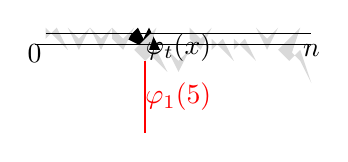
\begin{tikzpicture}[y=0.80pt, x=0.80pt, yscale=-1, inner sep=0pt, outer sep=0pt]
\path[fill=black] (41.6667,397.3333) -- (46.6667,392.3333) -- (51.6667,402.3333) --
  cycle;
\path[fill=black] (46.6667,402.3333) -- (51.6667,392.3333) -- (56.6667,402.3333)
  -- cycle;
\path[fill=gray!30] (5.0000,397.3333) -- (10.0000,392.3333) -- (15.0000,402.3333)
  -- (10.0000,397.3333) -- (5.0000,392.3333) -- cycle (15.0000,392.3333) --
  (20.0000,402.3333) -- (25.0000,392.3333) -- (20.0000,397.3333) -- (15.0000,392.3333)
  -- cycle (25.0000,392.3333) -- (30.0000,402.3333) -- (35.0000,392.3333) --
  (30.0000,397.3333) -- (25.0000,392.3333) -- cycle (35.0000,397.3333) --
  (40.0000,402.3333) -- (45.0000,392.3333) -- (40.0000,397.3333) -- (35.0000,392.3333)
  -- cycle (45.0000,402.3333) -- (50.0000,407.3333) -- (55.0000,392.3333) --
  (50.0000,397.3333) -- (45.0000,402.3333) -- cycle (50.0000,407.3333) --
  (55.0000,402.3333) -- (60.0000,412.3333) -- (55.0000,407.3333) -- (50.0000,402.3333)
  -- cycle (60.0000,402.3333) -- (65.0000,412.3333) -- (70.0000,402.3333) --
  (65.0000,407.3333) -- (60.0000,402.3333) -- cycle (70.0000,397.3333) --
  (75.0000,402.3333) -- (80.0000,392.3333) -- (75.0000,397.3333) -- (70.0000,392.3333)
  -- cycle (80.0000,402.3333) -- (85.0000,397.3333) -- (90.0000,407.3333) --
  (85.0000,402.3333) -- (80.0000,397.3333) -- cycle (90.0000,402.3333) --
  (95.0000,397.3333) -- (100.0000,407.3333) -- (95.0000,402.3333) -- (90.0000,397.3333)
  -- cycle (100.0000,392.3333) -- (105.0000,402.3333) -- (110.0000,392.3333) --
  (105.0000,397.3333) -- (100.0000,392.3333) -- cycle (110.0000,402.3333) --
  (115.0000,407.3333) -- (120.0000,392.3333) -- (115.0000,397.3333) --
  (110.0000,402.3333) -- cycle (115.0000,407.3333) -- (120.0000,402.3333) --
  (125.0000,417.3333) -- (120.0000,407.3333) -- (115.0000,402.3333) -- cycle;
\path[draw=red,line join=miter,line cap=butt,miter limit=4.00,line width=0.801pt]
  (50.0000,407.3333) -- (50.0000,440.0000) node[midway,right,red] {$\varphi_1(5)$};
\path[draw=black,line join=miter,line cap=butt,miter limit=4.00] (0.0000,400.0000) --
  (125.0000,400.0000);
\node[below] at (125.0000,400.0000) {$n$};
\node[below] at (0.0000,400.0000) {$0$};
\path[draw=black,line join=miter,line cap=butt,miter limit=4.00] (5.0000,395.0000) --
  (125.0000,395.0000) node[midway,below] {$\varphi_t(x)$};
\end{tikzpicture}
\end{document}